\subsection{Benutzeroberfläche}
Das Frontend des RadarSimulators verwendet das Framework JavaFX und wird über den SimulatorMainContentProvider bereitgestellt. Der SimulatorMainContentProvider enthält verschiedene Einstellungsmöglichkeiten und stellt Klassen, die die Funktionalität des   Benutzerinterface implementieren zur Verfügung. Diese Klassen heißen FXML Controller. Jeder FXML Controller ist mit einer FXML-Datei verknüpft, die die Anordnung der FXML Komponenten definiert. Der oberste FXML Controller des Radarsimulators ist der SimulatorMainController. 

Die Benutzeroberfläche besteht aus mehreren einzelnen Tabs, in denen die Funktionen des Simulators in unterschiedliche Bereiche eingeteilt werden. Jeder Tab hat einen Haupt FXML Controller. Wenn der Controller einen zu großen Funktionsumfang hat, kann Funktionalität auf weitere FXML Controller aufgeteilt werden. 

Da der SimulatorMainController der oberster FXML Controller ist, werden in ihm alle möglichen Tabs des Simulators vordefiniert und je nach Bedarf initialisiert. Welche Tabs geladen werden hängt davon ab, welcher Sensortyp und welche Asterixversion ausgewählt ist. Für jeden einzelnen Tab gibt es einen weiteren JavaFx Controller, in dem die Funktionalität der Oberfläche implementiert ist. Zwischen Backend und Frontend gibt es keine definierte Schnittstelle. Die Simulatorinstanz wird beim Erzeugen des Controllers an das Frontend übergeben. Das heißt die FXML Controller haben immer vollen Zugriff auf die Simulatorinstanz. Das ist nicht optimal, da Abhängigkeiten schnell unübersichtlich werden können und die Wartbarkeit des Systems erhöhen.

Um das genauer zu erläutern wird das Beipiel aus dem Sequenzdiagramm ABBL. Bit genauer betrachtet. Auf der GUI-Oberfläche wird nun ein Bitfehler hinzugefügt. Daraufhin reagiert der entsprechende actionListener. Er fügt den Bitfehler dem Model hinzu und sendet diesen über das Asterix-Interface an die Venus. Wenn die GUI Komponente das Model und den Sensor kontrolliert hat diese keine klare Aufgabe definiert. Bei einer Modularen Architektur ist es wichtig, dass jede Komponente „eine klar abgegrenzte Aufgabe“[Quelle 2] erfüllt. Somit ist diese Architektur fehlerhaft. Inwiefern die Funktion der View-Komponente verändert werden muss damit diese die Anforderungen einer modularen Architektur erfüllt wird in Kapitel 4.X geschildert.

\begin{figure}[h]
    \centering
    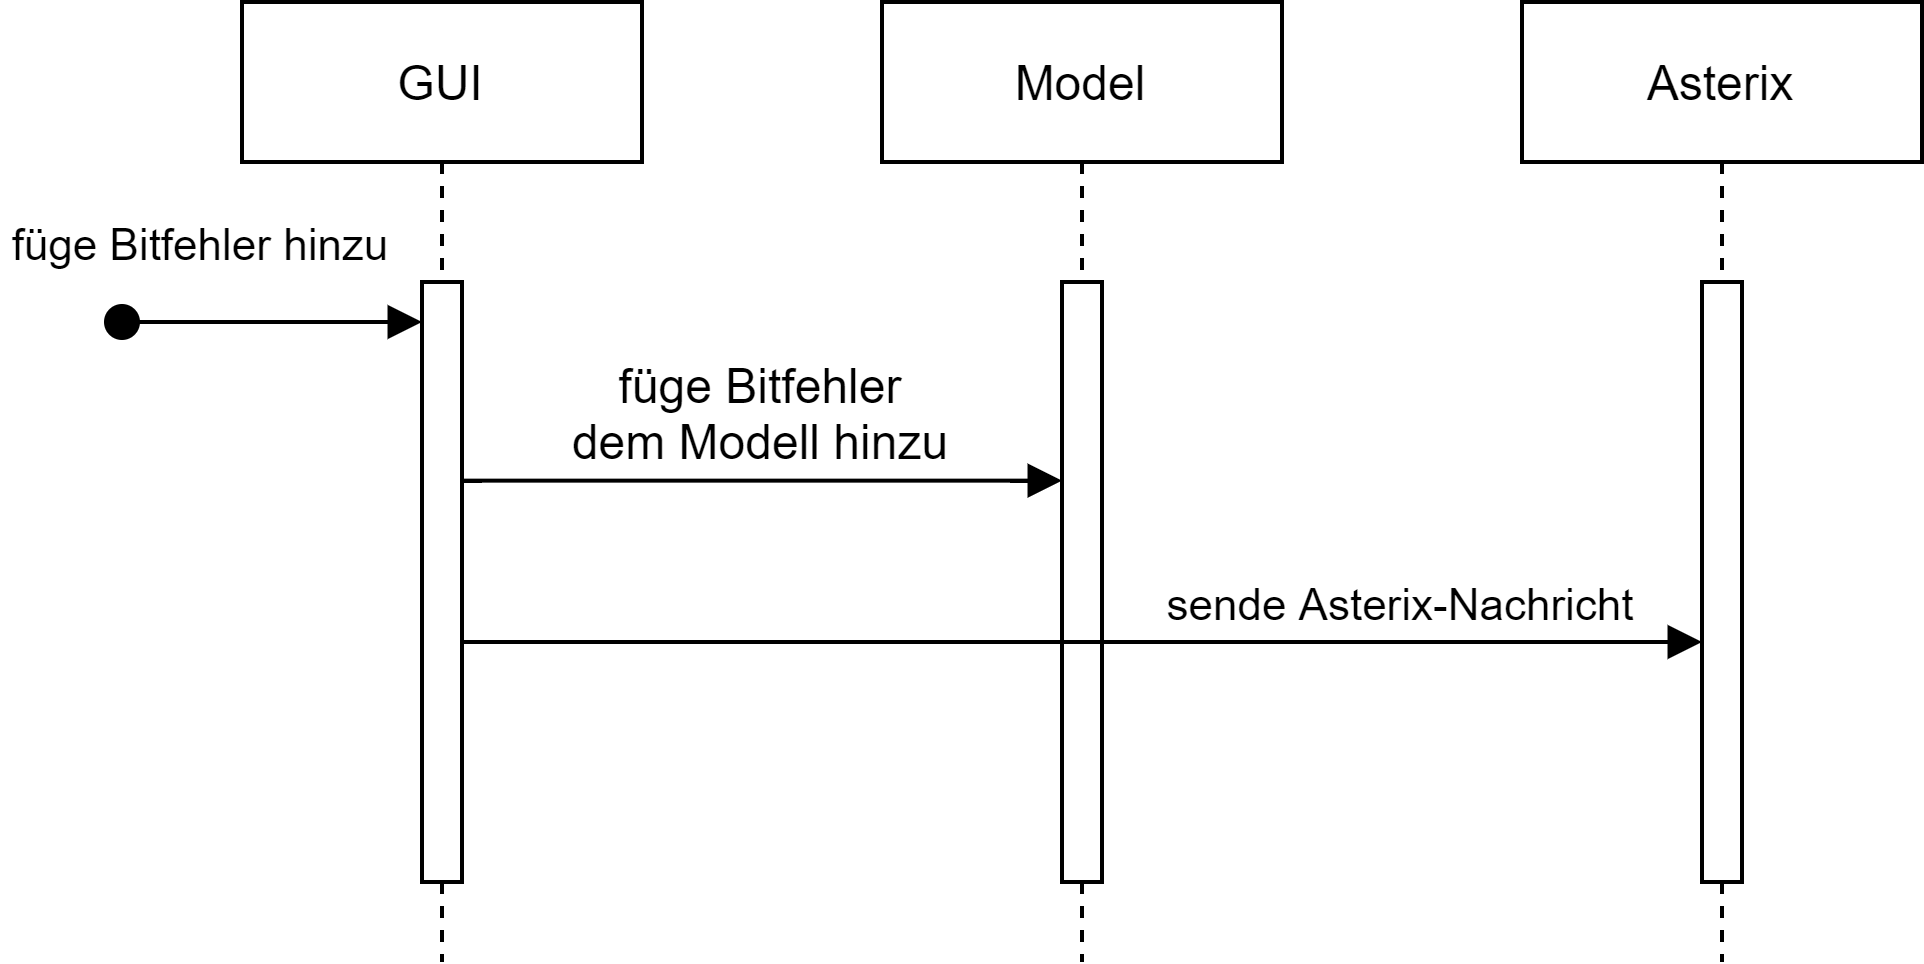
\includegraphics[width=0.8\textwidth]{content/assets/Kapitel3/AlterSimulator.png}
    \caption{UI - Alter Simulator}
\end{figure}

Weitere Optimierung bedarf es bei der Initialisierung der Tabs. Die späteren Anwendungen haben unterschiedlich viele Tabs. Die genaue Übersicht gibt es 
in ABBL. X

\begin{figure}[h]
    \centering
    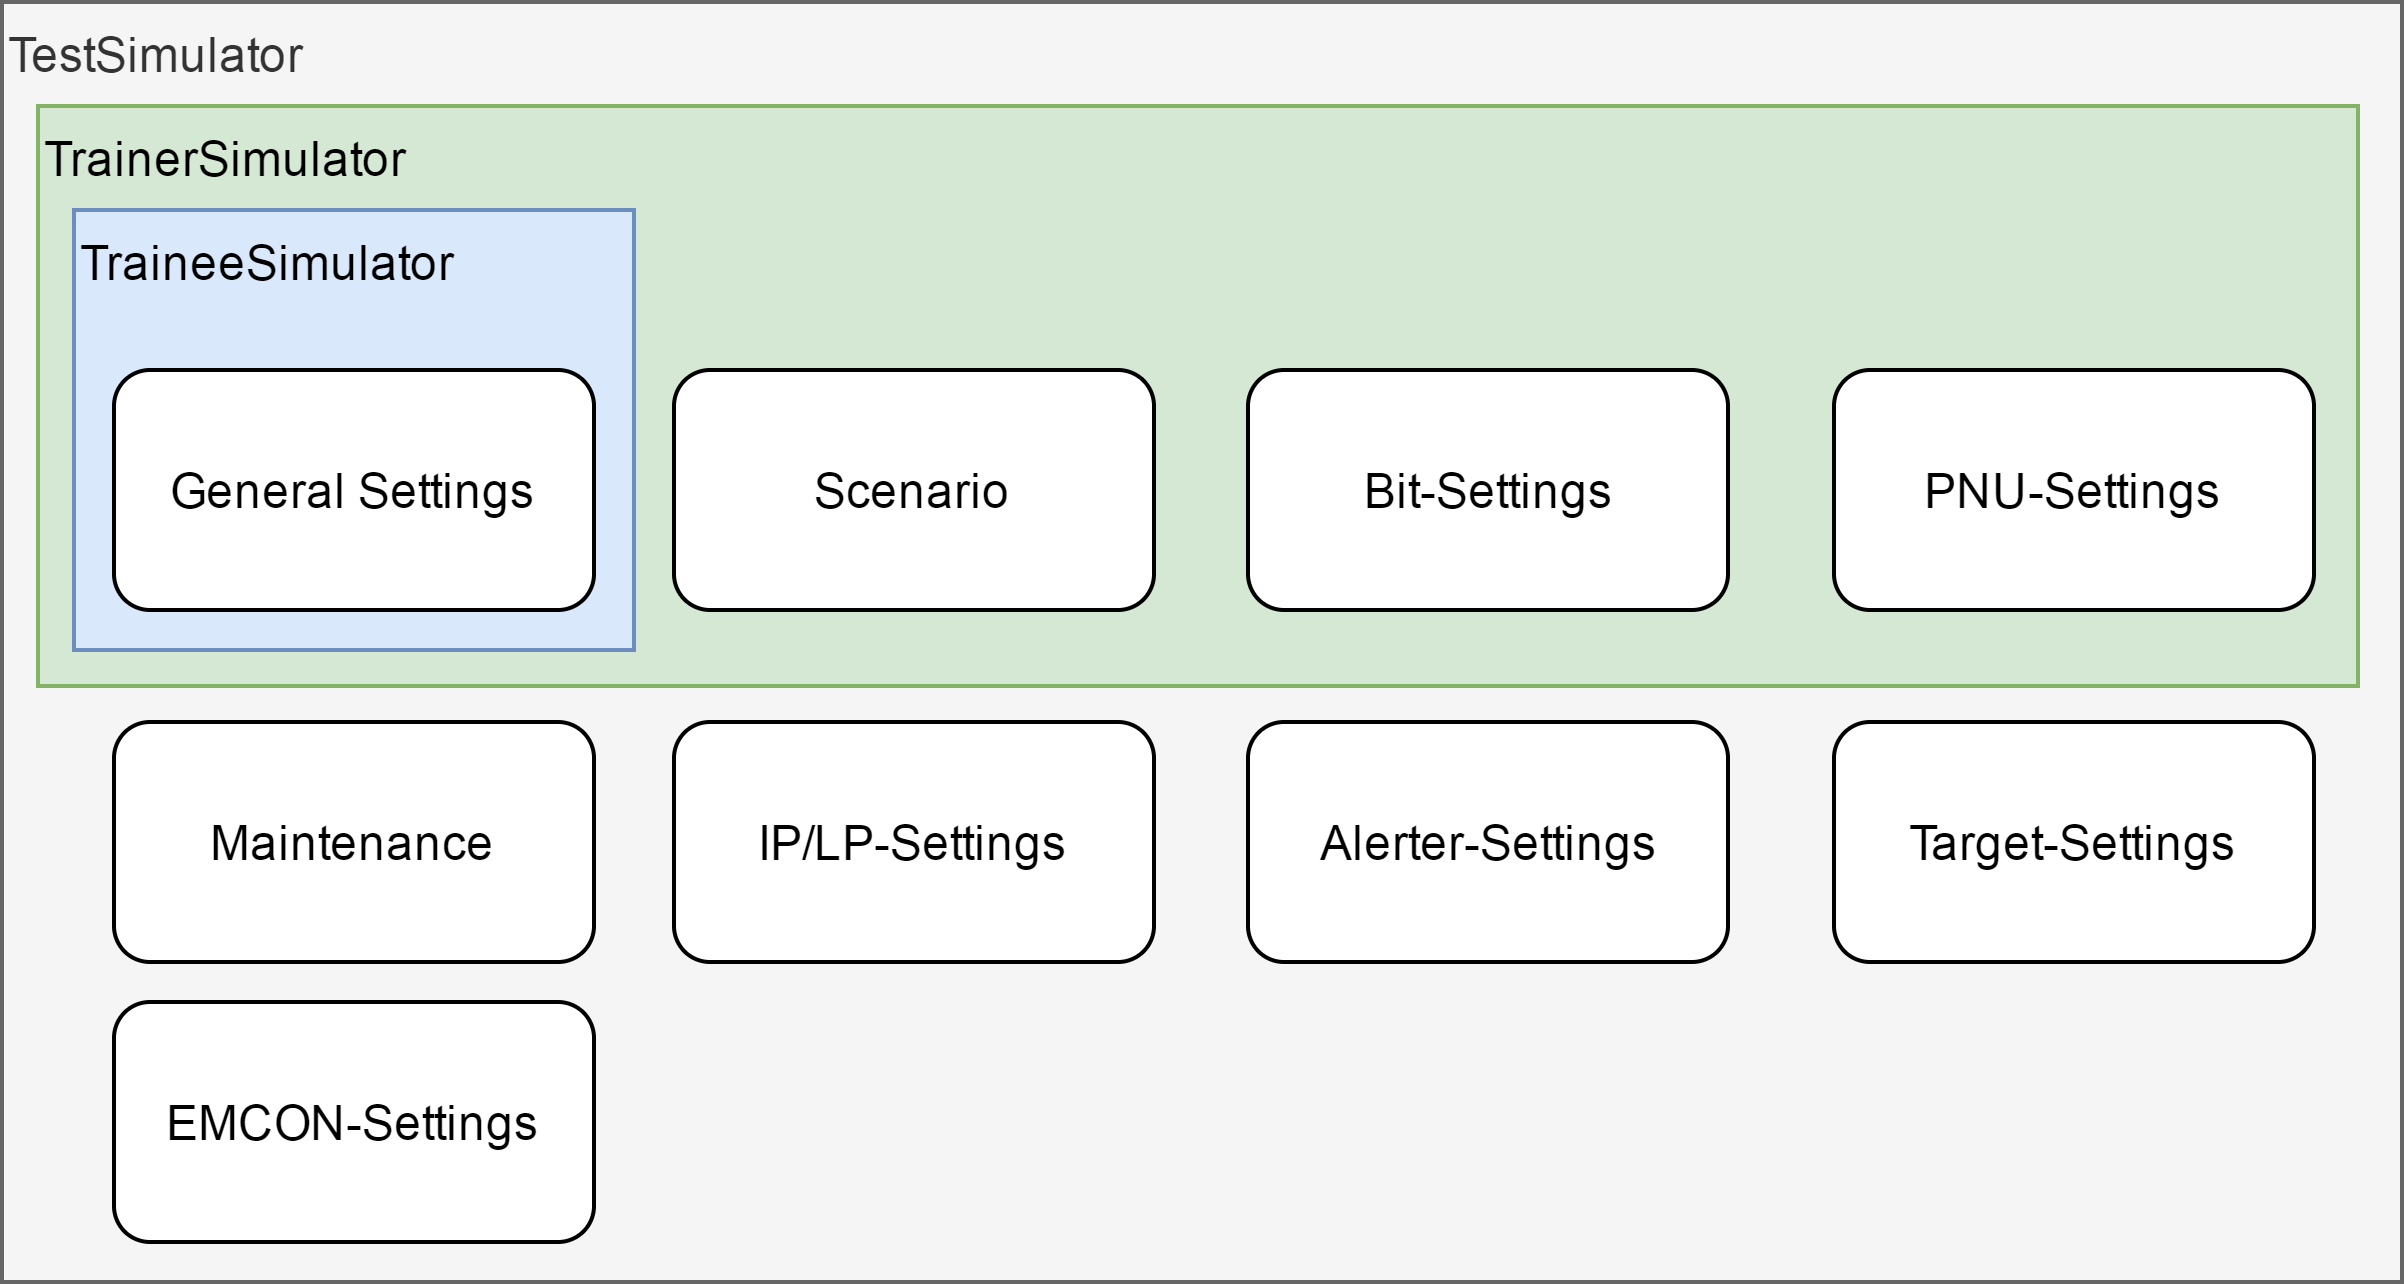
\includegraphics[width=0.8\textwidth]{content/assets/Kapitel3/TabsPerApp.png}
    \caption{UI - Alter Simulator}
\end{figure}

Deshalb ist es entweder notwendig für jede Anwendung einen separaten SimulatorMainController zu konfigurieren. Daraus würde redundanter Code entstehen, 
den man so gut es geht, vermeiden möchte. Die Alternative wäre eine allgemeinen SimulatorMainController, welcher alle verfügbaren Tabs im OSGi-Kontext 
lädt. Um das zu implementieren können Extension Points verwendet werden.
